%%%%%%%%%%%%%%%%%%%%%%%%%%%%%%%%%%%%%%%%%
% Lachaise Assignment
% LaTeX Template
% Version 1.0 (26/6/2018)
%
% This template originates from:
% http://www.LaTeXTemplates.com
%
% Authors:
% Marion Lachaise & François Févotte
% Vel (vel@LaTeXTemplates.com)
%
% License:
% CC BY-NC-SA 3.0 (http://creativecommons.org/licenses/by-nc-sa/3.0/)
% 
%%%%%%%%%%%%%%%%%%%%%%%%%%%%%%%%%%%%%%%%%

%----------------------------------------------------------------------------------------
%	PACKAGES AND OTHER DOCUMENT CONFIGURATIONS
%----------------------------------------------------------------------------------------

\documentclass{article}
\usepackage{graphicx}
\graphicspath{{images/}}
\usepackage{float} 
\usepackage{tikz, tikz-cd}
\usepackage{mathtools}
\usepackage{pgfplots}
\usetikzlibrary{spy}
\pgfplotsset{width=10cm,compat=1.18}
\input{structure.tex} % Include the file specifying the document structure and custom commands

%----------------------------------------------------------------------------------------
%	ASSIGNMENT INFORMATION
%----------------------------------------------------------------------------------------

\title{SINGLE-PHASE HALF-WAVE RECTIFIERS\\$R-L$ Load} % Title of the assignment

\author{Rodrigo Castillejos} % Author name and email address

\date{castillejosm.rodrigo@gmail.com} % University, school and/or department name(s) and a date

%----------------------------------------------------------------------------------------

\begin{document}

\maketitle % Print the title

%----------------------------------------------------------------------------------------
%	INTRODUCTION
%----------------------------------------------------------------------------------------

\section*{Introduction} % Unnumbered section
El rectificador de media onda con carga $R-L$ se muestra en la figura 1. Durante la conducción del diodo se puede desarrollar la siguiente ecuación:
\begin{figure}[H]
	\centering
	
\includegraphics[scale = 0.7]{figura1}
	\caption{Rectificador de media onda con carga $R-L$}
\end{figure}

% Math equation/formula
\begin{equation}
	L\frac{di}{dt} + Ri = \sqrt{2}V \sin(\omega t)
\end{equation}

o

\begin{equation}
	\frac{di}{dt} + \frac{R}{L}i = \frac{\sqrt{2}V}{L} \sin(\omega t)
\end{equation}

De la ecuación en (2) observamos que $P(x) = \frac{R}{L}$, por lo tanto, el factor de integración es:

\begin{align}
	\scalebox{1.5}{$\mu (x)= e^{\int \frac{L}{R} \, dx} = e^{\frac{R}{L}t}$}
\end{align}

Multiplicamos ambos lados de la ecuación en (2) por (3)
\begin{align}
	\underbrace{e^{\frac{R}{L}t}\frac{di}{dt} + e^{\frac{R}{L}t}\frac{R}{L} i} = e^{\frac{R}{L}t}\frac{\sqrt{2}V}{L}\sin \omega t\nonumber\\
	\frac{d}{dt}\left[ e^{\frac{R}{L}t} i \right] = e^{\frac{R}{L}t}\frac{\sqrt{2}V}{L}\sin \omega t 
\end{align}

Integramos ambos lados en la ecuación (4)
\begin{align}
	\int \frac{d}{dt}\left[ e^{\frac{R}{L}t} i \right] = \frac{\sqrt{2}V}{L} \int e^{\frac{R}{L}t}\sin \omega t 
\end{align}

\begin{align}
	e^{\frac{R}{L}t} i = \frac{\sqrt{2}V}{L} \int e^{\frac{R}{L}t}\sin \omega t 
\end{align}

\begin{info} % Information block
	Un tipo de ecuación diferencial de primer orden que ocurre con frecuencia en aplicaciones es la ecuación lineal. Recuerde que una ecuación lineal de primer orden es una ecuación expresada en la forma
	\begin{equation}
		a_1(x)\frac{dy}{dx} + a_0(x)y = b(x) \nonumber
	\end{equation}

	Donde $a_1(x)$, $a_0(x)$ y $b(x)$ dependen sólo de la variable independiente $x$, no de $y$. Esta ecuación se puede escribir en su forma estándar.
	\begin{equation}
		\frac{dy}{dx} + P(x)y = Q(x) \nonumber
	\end{equation}

	Donde $P(x)=a_0(x)/a_1(x)$ y $Q(x) = b(x)/a_1(x)$. Podemos resumir el método para resolver ecuaciones lineales como sigue:
	\begin{enumerate}
		\item Escriba la ecuación en su forma estándar
		\begin{equation}
			\frac{dy}{dx} + P(x)y = Q(x) \nonumber
		\end{equation}
		\item Calcule el factor de integración $\mu (x)$ por la fórmula
		\begin{equation}
			\mu (x) = e^{\int {P(x) dx}} \nonumber
		\end{equation}
		\item Multiplique la ecuación en la forma estándar por $\mu (x)$ y recordando que el lado derecho de la ecuación es sólo $\frac{d}{dx} [\mu (x)y]$, obtenemos 
			\begin{align}
				\underbrace{\mu (x) \frac{dy}{dx} + P(x)\mu (x)y} &= \mu (x)Q(x) \nonumber\\
				\frac{d}{dx}[\mu (x)y] &= \mu (x)Q(x) \nonumber	
			\end{align}

		\item Integra la última ecuación y resuelva para $y$ dividiendo en $\mu (x)$ para obtener
		\begin{align}
			y(x) = \frac{1}{\mu (x)}\left[ \int \mu(x)Q(x)dx + C \right] \nonumber
		\end{align}
	\end{enumerate}
\end{info}

Para encontrar la integral en (6) utilizamos la integración por partes, en específico la integración tabular como se muestra a continuación\\

\begin{tikzcd}[/tikz/cells={/tikz/nodes={shape=asymmetrical
			rectangle,text width=3cm,text height=2ex,text depth=0.3ex,align=center}}]
	e^{\frac{R}{L}t}\text{ y sus derivadas}	&	\sin \omega t \text{ y sus integrales}\\	
	e^{\frac{R}{L}t}  \arrow{dr}{+} & \sin \omega t \\
	\frac{R}{L}e^{\frac{R}{L}t} \arrow{dr}{-} & -\frac{1}{\omega}\cos \omega t \\
	\frac{R^{2}}{L^{2}}e^{\frac{R}{L}t} \arrow[r, shift left,"+"] & -\frac{1}{\omega^{2}}\sin \omega t
\end{tikzcd}

%\vspace{0.5cm}
Por lo tanto
\begin{align}
	\int e^{\frac{R}{L}t}\sin \omega t = -\frac{1}{\omega} e^{\frac{R}{L}t}\cos \omega t + \frac{R}{\omega ^{2} L} e^{\frac{R}{L}t} \sin \omega t - \frac{R^2}{\omega^{2} L^{2}}\int e^{\frac{R}{L}t} \sin \omega t \nonumber\\
		\int e^{\frac{R}{L}t}\sin \omega t + \frac{R^2}{\omega^{2} L^{2}}\int e^{\frac{R}{L}t} \sin \omega t = -\frac{1}{\omega} e^{\frac{R}{L}t}\cos \omega t + \frac{R}{\omega ^{2} L} e^{\frac{R}{L}t} \sin \omega t\nonumber\\
	\left( 1 + \frac{R^2}{\omega^{2}L^2} \right) \int e^{\frac{R}{L}t}\sin \omega t =  -\frac{1}{\omega} e^{\frac{R}{L}t}\cos \omega t + \frac{R}{\omega ^{2} L} e^{\frac{R}{L}t} \sin \omega t\nonumber\\
	\left(\frac{R^2 + \omega^{2}L^2}{\omega^{2}L^2} \right) \int e^{\frac{R}{L}t}\sin \omega t =  -\frac{1}{\omega} e^{\frac{R}{L}t}\cos \omega t + \frac{R}{\omega ^{2} L} e^{\frac{R}{L}t} \sin \omega t\nonumber\\
	\int e^{\frac{R}{L}t}\sin \omega t = -\frac{\omega^{2}L^2}{R^2 + \omega^{2}L^2}\left( \frac{1}{\omega}\right) e^{\frac{R}{L}t}\cos \omega t +  \frac{\omega^{2}L^2}{R^2 + \omega^{2}L^2}\left( \frac{R}{\omega^{2}L} \right)e^{\frac{R}{L}t}\sin \omega t\nonumber + C
\end{align}
Así
\begin{align}
	\int e^{\frac{R}{L}t}\sin \omega t = \frac{RL}{R^2 + \omega^{2}L^2}e^{\frac{R}{L}t}\sin \omega t -\frac{\omega L^2}{R^2 + \omega^{2}L^2}e^{\frac{R}{L}t} \cos \omega t + C
\end{align}

La sustitución de (7) en (6) produce
\begin{align}
	e^{\frac{R}{L}t}i = \frac{\sqrt{2}V}{L}\left[ \frac{RL}{R^2 + \omega^{2}L^2}e^{\frac{R}{L}t}\sin \omega t -\frac{\omega L^2}{R^2 + \omega^{2}L^2}e^{\frac{R}{L}t} \cos \omega t + C\right]\nonumber\\
	e^{\frac{R}{L}t}i = \sqrt{2}V\left[ \frac{R}{R^2 + \omega^{2}L^2}e^{\frac{R}{L}t}\sin \omega t -\frac{\omega L}{R^2 + \omega^{2}L^2}e^{\frac{R}{L}t} \cos \omega t + A \right]\nonumber\\
	i = \sqrt{2}V\left[ \frac{R}{R^2 + \omega^{2}L^2}\sin \omega t -\frac{\omega L}{R^2 + \omega^{2}L^2} \cos \omega t + Ae^{-\frac{R}{L}t}\right]
\end{align}
%----------------------------------------------------------------------------------------
%	PROBLEM 1
%----------------------------------------------------------------------------------------

\begin{info}
	Demostración de que $A\sin \theta + B\sin\cos \theta = C \sin (\theta + \alpha)$\\
	Nos basamos en la identidad trigonométrica de la suma de ángulos:
	\begin{align}
		C\sin(\theta + \alpha) &= C \left[ (\sin \theta) (\cos \alpha) + (\sin \alpha) (\cos \theta) \right]\nonumber\\
		&= C(\sin \theta) (\cos \alpha) + C(\sin \alpha) (\cos \theta)\nonumber\\
		&= \underbrace{C\cos \alpha}_{A} \sin \theta + \underbrace{C\sin \alpha}_{B}\cos \theta \nonumber \\
		&= A \sin \theta + B \cos \theta\nonumber
	\end{align}

Donde 
\begin{align}
	C\cos \alpha = A\\
	C\sin \alpha = B
\end{align}

Basándonos en la identidad del cociente obtenemos 
\begin{align}
	\tan \alpha &= \frac{C\sin \alpha}{C\cos \alpha} = \frac{B}{A}\nonumber \therefore\\
	\alpha &= \tan^{-1} \frac{B}{A}
\end{align}

Si elevamos al cuadrado ambos miembros de la ecuación (9) y (10) y las sumamos entre sí obtenemos
\begin{align}
	C^2 \cos^2 \alpha  + C^2 \sin^2\alpha &= A^2 + B^2\nonumber\\
	C^2 \left[ \sin^2 \alpha + \cos^2 \alpha \right] &= A^2 + B^2\nonumber\\
	C^2 &= A^2 + B^2\nonumber\\
	C &= \sqrt{A^2 + B^2}
\end{align}
\end{info}

La ecuación en (8) se puede expresar como
\begin{align}
	i = \frac{\sqrt{2}V \sin(\omega t - \alpha)}{\sqrt{R^2 + (\omega L)^2}} + Ae^{-\frac{R}{L}t}
\end{align}

Donde
\begin{align}
	\alpha = \tan^{-1}\frac{\omega L}{R}
\end{align}


Donde 
\begin{align}
	\frac{R}{R^2 + \omega^{2}L^2}\sin \omega t -\frac{\omega L}{R^2 + \omega^{2}L^2} \cos \omega t &= \sqrt{\frac{R^2}{(R^2 + \omega^{2}L^2)^2} + \frac{\omega^{2}L^2}{(R^2 + \omega^{2}L^2)^2}}\sin (\omega t - \alpha)\nonumber\\
	&=\sqrt{\frac{R^2+\omega^{2}L^2}{(R^2 + \omega^{2}L^2)^2} }\sin (\omega t - \alpha)\nonumber\\
	&=\frac{\sin(\omega t - \alpha)}{\sqrt{R^2 + \omega^{2}L^2}}\nonumber
\end{align}

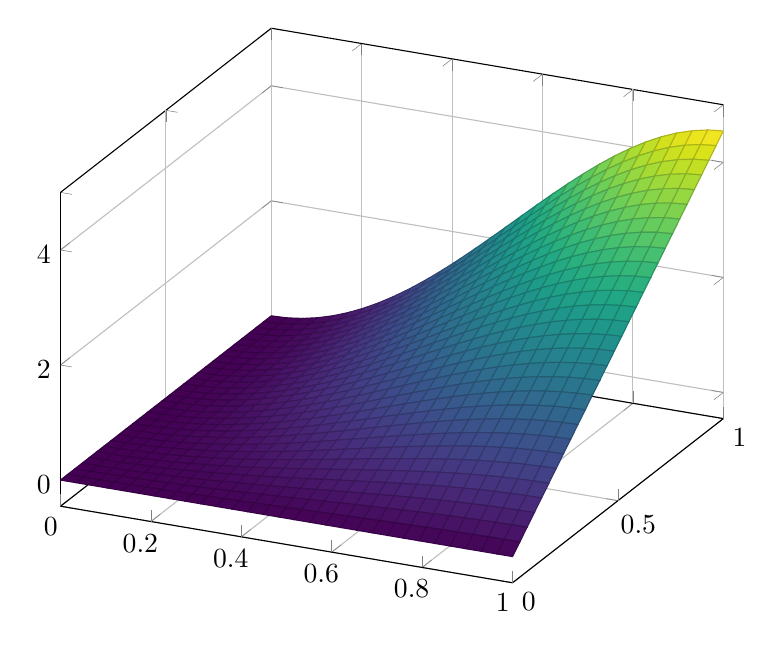
\begin{tikzpicture}
	\begin{axis}[
		grid=major,
		colormap/viridis,
		]
		\addplot3 [
		surf,
		samples=30,
		domain=0:1,
		] {5*x*sin(2*deg(x)) * y};
	\end{axis}
\end{tikzpicture}

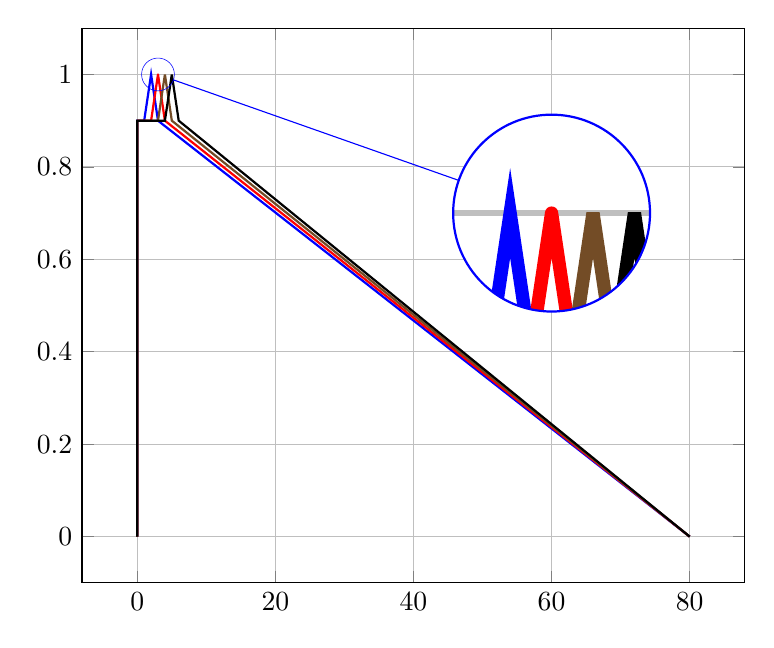
\begin{tikzpicture}[spy using outlines=
	{circle, magnification=6, connect spies}]
	\begin{axis}[no markers,grid=major,
		every axis plot post/.append style={thick}]
		\addplot coordinates
		{(0, 0) (0, 0.9) (1, 0.9) (2, 1) (3, 0.9) (80, 0)};
		\addplot+ [line join=round] coordinates
		{(0, 0) (0, 0.9) (2, 0.9) (3, 1) (4, 0.9) (80, 0)};
		\addplot+ [line join=bevel] coordinates
		{(0, 0) (0, 0.9) (3, 0.9) (4, 1) (5, 0.9) (80, 0)};
		\addplot+ [miter limit=5] coordinates
		{(0, 0) (0, 0.9) (4, 0.9) (5, 1) (6, 0.9) (80, 0)};
		\coordinate (spypoint) at (3,1);
		\coordinate (magnifyglass) at (60,0.7);
	\end{axis}
	\spy [blue, size=2.5cm] on (spypoint)
	in node[fill=white] at (magnifyglass);
\end{tikzpicture}
%----------------------------------------------------------------------------------------
%	PROBLEM 2
%----------------------------------------------------------------------------------------

\end{document}
